\documentclass{article}
\usepackage{amsmath}
\usepackage{xcolor}
\usepackage{gensymb}
\usepackage{ragged2e}
\usepackage{graphicx}
\usepackage{gensymb}
\usepackage{mathtools}
\newcommand{\mydet}[1]{\ensuremath{\begin{vmatrix}#1\end{vmatrix}}}
\providecommand{\brak}[1]{\ensuremath{\left(#1\right)}}
\providecommand{\norm}[1]{\left\lVert#1\right\rVert}
\newcommand{\solution}{\noindent \textbf{Solution: }}
\newcommand{\myvec}[1]{\ensuremath{\begin{pmatrix}#1\end{pmatrix}}}
\let\vec\mathbf 


\begin{document}
\begin{center}
        \textbf\large{CHAPTER-7 \\ TRIANGLES}
\end{center}
\section{Exercise 7.1}
Q3. $AD$ and $BC$ are equal perpendiculars to a line segment $AB$. Show that $CD$ bisects $AB$.\\
\textbf{Construction}\\
\begin{figure}[h]
	\begin{center}
		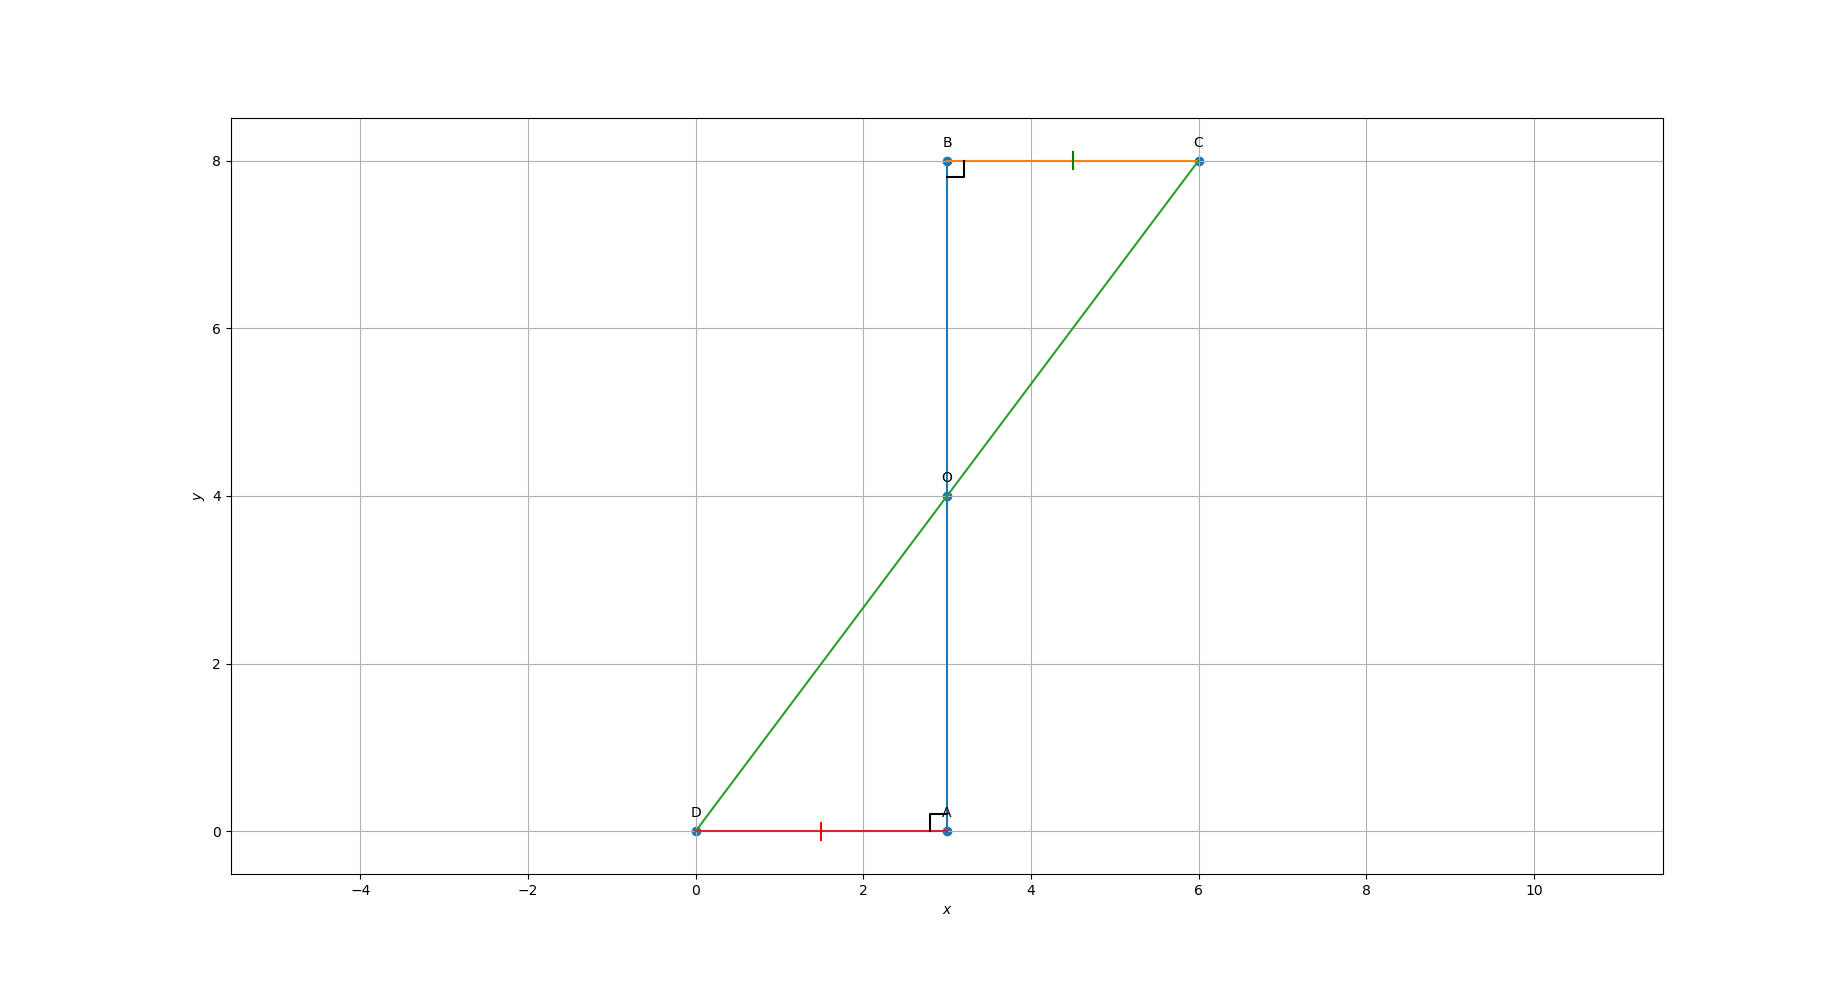
\includegraphics[width=\columnwidth]{figs/Figure1.png}
	\end{center}
	\label{fig:Fig1}
\end{figure}
The input parameters for construction are shown in \ref{tab:Table1}:\\
\begin{table}[h]
	  \centering
	  \begin{tabular}{|p{3cm}|p{3cm}|p{3cm}|}
\hline                                        
	\textbf{Symbol} & \textbf{Values} & \textbf{Description} \\                                          
\hline                                 
	a & 3 & $AD=BC$ \\        
\hline                                    
	b & 4 & $AB$ \\    
\hline                      
	$\vec{e}_1$ & $\myvec{1\\0}$ & basis vector \\
\hline
\end{tabular}

	  \caption{Parameters}
	  \label{tab:Table1}
\end{table}
\pagebreak
\begin{align}
	\vec{A} = a\vec{e_1},\vec{B} = \myvec{a\\b},\vec{C} = \myvec{2a\\b},\vec{D} = \myvec{0\\0}
\end{align}
\solution
Given
\begin{align}
	\vec{D}-\vec{A}&=\vec{B}-\vec{C}\\
	\angle DAB &= \angle CBA=90\degree
\end{align}
\textbf{To Prove:}\\
\begin{align}
	\vec{C}-\vec{O}&=\vec{O}-\vec{D}
\end{align}
\textbf{Proof:}\\
Consider linesegment $DC$\\
Let $\vec{O}$ represent the Midpoint of $DC$
\begin{align}
	\vec{O}&=\frac{1}{2}(\vec{C}+\vec{D})\\
	\implies &= \frac{1}{2}\myvec{6\\8}+\frac{1}{2}\myvec{0\\0}\\
	\implies &= \frac{1}{2}\myvec{6\\8}\\
		 &=\myvec{3\\4}
		 \label{eq:1}\\
\end{align}
\begin{align}
	\text { Since $AB\perp DA$, $AB$ is parallel to $x=0$ }\\
	\text { Equation of $AB$ is defined as $x=3$}\\
	\label{eq:2}\\
\end{align}
from $\eqref{eq:1}$ and $\eqref{eq:2}$
$\vec{O}$ lies on linesegment $CD$ and line $DC$ intersects $BA$ at its midpoint $O$.
\begin{align}
\vec{C}-\vec{O}=\vec{O}-\vec{D}
\end{align}
\end{document}
